%%% TeX-command-extra-options: "-shell-escape"
%\documentclass[aspectratio=169]{beamer}
\documentclass[10pt]{beamer}

% Package section
\usepackage[english]{babel}
\usepackage[utf8]{inputenc}
\usepackage[T1]{fontenc}

\usepackage{listings}
\usepackage{graphicx}
\usepackage{color}
\usepackage[sfdefault, light, lining]{FiraSans}

%\usepackage{minted}
%\usepackage{hyperref}
%\usepackage{sourcecodepro}
\usepackage{courier}
\usepackage{gitdags}
\usepackage{subcaption}
\usepackage{xcolor-solarized}

\usepackage[version=4]{mhchem}
\usepackage{siunitx}
\sisetup{detect-all=true}



% Colors
% ======
% \definecolor{bg_gray}{HTML}{e2e1de}
%\definecolor{bg_gray}{HTML}{e8e6e3}
\colorlet{bg_gray}{black!10}
\definecolor{TolDarkPurple}{HTML}{332288}
\definecolor{TolDarkBlue}{HTML}{6699CC}
\definecolor{TolLightBlue}{HTML}{88CCEE}
\definecolor{TolLightGreen}{HTML}{44AA99}
\definecolor{TolDarkGreen}{HTML}{117733}
\definecolor{TolDarkBrown}{HTML}{999933}
\definecolor{TolLightBrown}{HTML}{DDCC77}
\definecolor{TolDarkRed}{HTML}{661100}
\definecolor{TolLightRed}{HTML}{CC6677}
\definecolor{TolLightPink}{HTML}{AA4466}
\definecolor{TolDarkPink}{HTML}{882255}
\definecolor{TolLightPurple}{HTML}{AA4499}


% Gruvbox
% -------
\definecolor{gb_bg}{HTML}{282828}
\definecolor{gb_darkred}{HTML}{cc241d}
\definecolor{gb_darkgreen}{HTML}{98971a}
\definecolor{gb_darkyellow}{HTML}{d79921}
\definecolor{gb_darkblue}{HTML}{458588}
\definecolor{gb_darkpurple}{HTML}{b16286}
\definecolor{gb_darkteal}{HTML}{689d6a}
\definecolor{gb_darkgray}{HTML}{a89984}

\definecolor{gb_gray}{HTML}{928374}
\definecolor{gb_red}{HTML}{fb4934}
\definecolor{gb_green}{HTML}{b8bb26}
\definecolor{gb_yellow}{HTML}{fabd2f}
\definecolor{gb_blue}{HTML}{83a598}
\definecolor{gb_purple}{HTML}{d3869b}
\definecolor{gb_teal}{HTML}{8ec07c}
\definecolor{gb_fg}{HTML}{ebdbb2}

\hypersetup{colorlinks,linkcolor=,urlcolor=TolLightPink}
%\hypersetup{
%    linkcolor = \color{TolDarkPink},
%    urlcolor = \color{TolDarkPink},
%    allcolors= \color{TolDarkPink}
%}

% Tikz settings
% -------------
\tikzset{
  labelst/.style={
    draw,
    node distance = 1.4em,
    drop shadow   = {opacity=0.15},
    font          = \fontfamily{lmtt}\selectfont\small,
    shape                        = rounded rectangle,
    minimum height               = 1.6em,
    minimum width                = 2em,
    draw                         = solarized-base01,
    very thick,
  },
  labelnode/.style={
    labelst,
    rounded rectangle arc length = 90,
  },
  refnode/.style={
    labelst,
    rectangle,
  },
  linenode/.style={
    draw = solarized-base01,
    dashed,
    very thick,
  },
  arrownoder/.style={
    thick,
    -Latex,
    draw = solarized-base01,
  },
  arrownodel/.style={
    semithick,
    Latex-,
    draw = gray,
  }
}


\lstset{numbers=right,
  numberstyle=\tiny,
  basicstyle=\footnotesize\ttfamily,
  breaklines=true,
  numbersep=1.5ex,
  xleftmargin=2ex,
  xrightmargin=2ex,
  framexleftmargin=1ex,
  framexrightmargin=1ex,
  backgroundcolor=\color{bg_gray}}
%\lstset{framextopmargin=50pt,frame=bottomline}


% Python programming
% ------------------

% Custom colors
\definecolor{deepblue}{rgb}{0,0,0.5}
\definecolor{deepred}{rgb}{0.6,0,0}
\definecolor{deepgreen}{rgb}{0,0.5,0}


% Python style for highlighting
\newcommand\pythonstyle{\lstset{
language=Python,
numbers=right,
numberstyle=\tiny,
basicstyle=\footnotesize\ttfamily,
otherkeywords={self,as},             % Add keywords here
keywordstyle=\bfseries\color{gb_red},
emph={MyClass,__init__},          % Custom highlighting
emphstyle=\bfseries\color{gb_blue},    % Custom highlighting style
stringstyle=\color{gb_green},
showstringspaces=false,            %
commentstyle=\itshape\color{gb_gray},
numbersep=1.5ex,
xleftmargin=2ex,
xrightmargin=2ex,
framexleftmargin=1ex,
framexrightmargin=1ex,
backgroundcolor=\color{bg_gray}
}}

% Fortran style for highlighting
\newcommand\fortranstyle{\lstset{
language=Fortran,
numbers=right,
numberstyle=\tiny,
basicstyle=\footnotesize\ttfamily,
%otherkeywords={program},             % Add keywords here
keywordstyle=\bfseries\color{gb_red},
emph={program,end,subroutine,module,function,contains},          % Custom highlighting
emphstyle=\bfseries\color{gb_blue},    % Custom highlighting style
stringstyle=\color{gb_darkgreen},
showstringspaces=false,            %
commentstyle=\itshape\color{gb_gray},
numbersep=1.5ex,
xleftmargin=2ex,
xrightmargin=2ex,
framexleftmargin=1ex,
framexrightmargin=1ex,
backgroundcolor=\color{bg_gray}
}}

% Makefile style for highlighting
\newcommand\makefilestyle{\lstset{
    language=[gnu] make,
    numbers=right,
    numberstyle=\tiny,
    basicstyle=\footnotesize\ttfamily,
    % otherkeywords={program},             % Add keywords here
    keywordstyle=\bfseries\color{gb_red},
    emph={program,end,subroutine,module,function,contains},          % Custom highlighting
    emphstyle=\bfseries\color{gb_blue},    % Custom highlighting style
    stringstyle=\color{gb_darkgreen},
    showstringspaces=false,            %
    commentstyle=\itshape\color{gb_gray},
    numbersep=1.5ex,
    xleftmargin=2ex,
    xrightmargin=2ex,
    framexleftmargin=1ex,
    framexrightmargin=1ex,
    backgroundcolor=\color{bg_gray}
  }}


% Python environment
\lstnewenvironment{python}[1][]
{
\pythonstyle
\lstset{#1}
}
{}

% Fortran
\lstnewenvironment{fortran}[1][]
{
\fortranstyle
\lstset{#1}
}
{}

% makefile
\lstnewenvironment{makefile}[1][]
{
  \makefilestyle
  \lstset{#1}
}
{}

\newcommand\fortraninline[1]{{\fortranstyle\lstinline!#1!}}

% Python for external files
\newcommand\pythonexternal[2][]{{
\pythonstyle
\lstinputlisting[#1]{#2}}}

% Python for inline
\newcommand\pythoninline[1]{{\pythonstyle\lstinline!#1!}}



\usetheme[progressbar=foot]{metropolis}           % Use metropolis theme
\metroset{block=fill}

% New commands and other simplification stuff
\newcommand{\ccpq}{CC(\textit{P};\textit{Q})}
%\let\OldTexttt\texttt
\newcommand{\textco}[1]{\colorbox{bg_gray}{\texttt{#1}}}

\title{Driving Scientific Computations with \texttt{Make}}
\date{\today}
\author{J. Emiliano Deustua}
\institute{Miller's Group \\ Caltech}

\begin{document}
  \maketitle

  \begin{frame}[fragile]
    \frametitle{Notation used in this presentation}
    \begin{block}{Shell commands}<+->
      Commands in the command line are prefixed with \texttt{\$}, e.g.
\begin{lstlisting}[numbers=none,backgroundcolor=\color{gray!10}]
$ mkdir my_foobar_dir
$ vim my_foobar_file
\end{lstlisting}
    \end{block}

    \begin{block}{Placeholders}<+->
      Placeholders for files or variables will be surrounded by \texttt{[]}, e.g.
\begin{lstlisting}[numbers=none,backgroundcolor=\color{gray!10}]
$ cat [A FILE] > [ANOTHER FILE]
\end{lstlisting}
    \end{block}
  \end{frame}


  \begin{frame}{What is \texttt{Make}?}
    \begin{itemize}[<+->]
    \item \textco{make} is a \alert{build automation system tool} designed to build
      binary executables and libraries from source files.

    \item Originally written by Stuart Feldman in 1976 (\alert{45 years old!}) for the UNIX OS.

    \item Nowadays widely used for building most GNU and open source software
      in Linux hand-to-hand with \textco{autoconf}, \textco{automake}, and
      \textco{cmake}. \alert{Very likely you have used it before.}

    \item Pretty much available in any modern Linux
      distributions as \textco{GNU Make}.

    \item Full manual
      \url{https://www.gnu.org/software/make/manual/make.html}
  \end{itemize}

  \end{frame}


  \begin{frame}[fragile]
    \frametitle{How does it work?}

    \begin{enumerate}[<+->]
    \item \textco{make} parses a \textco{Makefile} consisting of a set of \textbf{file-creation rules}
      which completely \alert{defines its behavior}.
    \item generates a \alert{dependency graph}
    \item \alert{runs recipes} following the graph until \alert{all files
      have been generated} and \alert{all timestamps follow the dependency order}.
    \end{enumerate}

    \visible<+->{
    \begin{figure}
      \centering
      \begin{tikzpicture}[
        level 1/.style={sibling distance=10em},
        level 2/.style={sibling distance=4em},
        level 3/.style={sibling distance=2em},
        every node/.style={labelnode, fill=solarized-green!20}]
        \node[fill=solarized-red!20]{parser.x}
        child{node (main_node) {main.o}
          child{node{main.c}}
          child{node{main.h}}}
        child{node{ast.o}
          child{node (ast_node) {ast.h}}
          child{node{ast.c}}};

        \path (main_node) edge (ast_node);

      \end{tikzpicture}
      \caption{Example file dependency graph}
    \end{figure}
    }

    \visible<+->{
    \begin{center}
      \textbf{In general, any set of files and rules works!}
    \end{center}
    }
  \end{frame}


  \begin{frame}[fragile]
    \frametitle{A \texttt{Makefile} Example}
\begin{makefile}
# Comments start with # as in bash
# Usually, one begins a file by setting some variables.
# For example:
COMPILER := gcc
LINKER := gcc

# The body of the Makefile consists of a set of rules
# which follow the following syntax:

# [TARGET] ... : [PREREQUISITES] ...
#    [RECIPE]

parser.x: main.o ast.o
    $(LINKER) main.o ast.o

main.o: main.h main.c ast.h
    $(COMPILER) -c main.c

ast.o: ast.h ast.c
    $(COMPILER) -c ast.o
\end{makefile}
\end{frame}


\begin{frame}[fragile]{Decomposing a Rule Entry}
\begin{makefile}
[TARGET]: [PREREQUISITES]
    [RECIPE]
\end{makefile}
  \begin{itemize}
    \item<+-> A \textco{[TARGET]} usually the name of the file that is generated by
      the \textco{[RECIPE]}. Can also be a phony target (will discuss later).\\

    \item<+-> A \textco{[PREREQUISITE]]} is a file the \textco{[RECIPE]} depends
      on (can be a file created by another rule).\\

    \item<+-> A \textco{[RECIPE]} is a shell command that \textco{make} executes
      to generate the \textco{[TARGET]}.

  \end{itemize}

  \begin{alertblock}{Note}<+->
    \begin{itemize}
    \item \textco{[RECIPE]} lines must be prefixed by a tab character
    \item Multiple \textco{[RECIPE]} lines are allowed, but they are sent to different shells if
        not terminated by a backslash.
    \end{itemize}
  \end{alertblock}
\end{frame}


\begin{frame}[fragile]{\texttt{Make} Execution}
  Once a \textco{Makefile} is written, \textco{make} can be executed in a shell,
  in the same directory as the \textco{Makefile}
  \begin{lstlisting}
$ make
\end{lstlisting}
  This will:
  \begin{enumerate}[<+->]
  \item load the rules
  \item create the dependency graph
    \item and start executing the
      recipes, beginning with the first rule in the \textco{Makefile}.
    \end{enumerate}

  \begin{exampleblock}{Tip}<+->
  One can select a particular \textco{[TARGET]} to execute by passing it to
  \textco{make}, as so
\begin{lstlisting}
$ make [TARGET]
\end{lstlisting}
\end{exampleblock}

\end{frame}


  \begin{frame}[fragile]{\texttt{Make} basic features}
    \textco{Make} is loaded with a bunch of functions. For example,
    one can load paths from the file-system,
\begin{makefile}
PATHS := $(wildcard *.txt)
\end{makefile}
    \pause

    do pattern substitutions,
\begin{makefile}
PATHS := $(wildcard *.txt)
NEW_PATHS := $(patsubst %.txt,%.text,$(PATHS))$
\end{makefile}
    \pause

    call shell commands,
\begin{makefile}
PATHS := $(shell seq 1 10)
INPUTS := $(addsuffix .inp,$(PATHS))
\end{makefile}
    \pause

    and much more, including conditionals and loops\\
    {\tiny \url{https://www.gnu.org/software/make/manual/html_node/Functions.html}}.
  \end{frame}

  \begin{frame}[fragile]{\texttt{Make} basic features}
    \textco{Make} also generates a set of automatic variables that help in
    writing rules. For example,
    one can load the name of the target and prerequisites
\begin{makefile}
requisites.txt: A couple of words
    echo $^ > $@

A couple of words:
\end{makefile}
    where \textco{\$\^} holds all prerequisites and \textco{\$@}, the target.
    \pause

    One can also write rules based on patterns, as so,
\begin{makefile}
%.o: %.c
    gcc -c $< -o $@
\end{makefile}
    which allows for writing generic recipes a file type. In this case
    \textco{\$<} holds the name of the first prerequisite.

    {\tiny
      \url{https://www.gnu.org/software/make/manual/html_node/Automatic-Variables.html} \\
      \vspace{-2ex}
      \url{https://www.gnu.org/software/make/manual/html_node/Pattern-Intro.html}}

  \end{frame}


\begin{frame}[fragile]{\texttt{PHONY} targets}
  Sometimes it is useful to write rules which are not associated with a file.
  For example,
\begin{makefile}
clean:
    rm *.o
\end{makefile}
  \pause
  Normally, this rule will try to find a file named \textco{clean} in the
  working directory, and if it exists the rule would not be executed. To let
  \textco{Make} know this is a dummy rule one can use the \textco{.PHONY} declaration:
\begin{makefile}
.PHONY: clean

clean:
    rm *.o
\end{makefile}
\end{frame}


\begin{frame}[fragile]{An example use in scientific: \ce{H2} dissociation}
  Let's write a real world example \textco{Makefile}: the potential energy surface
  of the dissociation of \ce{H2} computed with \texttt{Psi4} at the CCSD/cc-pVDZ level.
  \begin{center}
    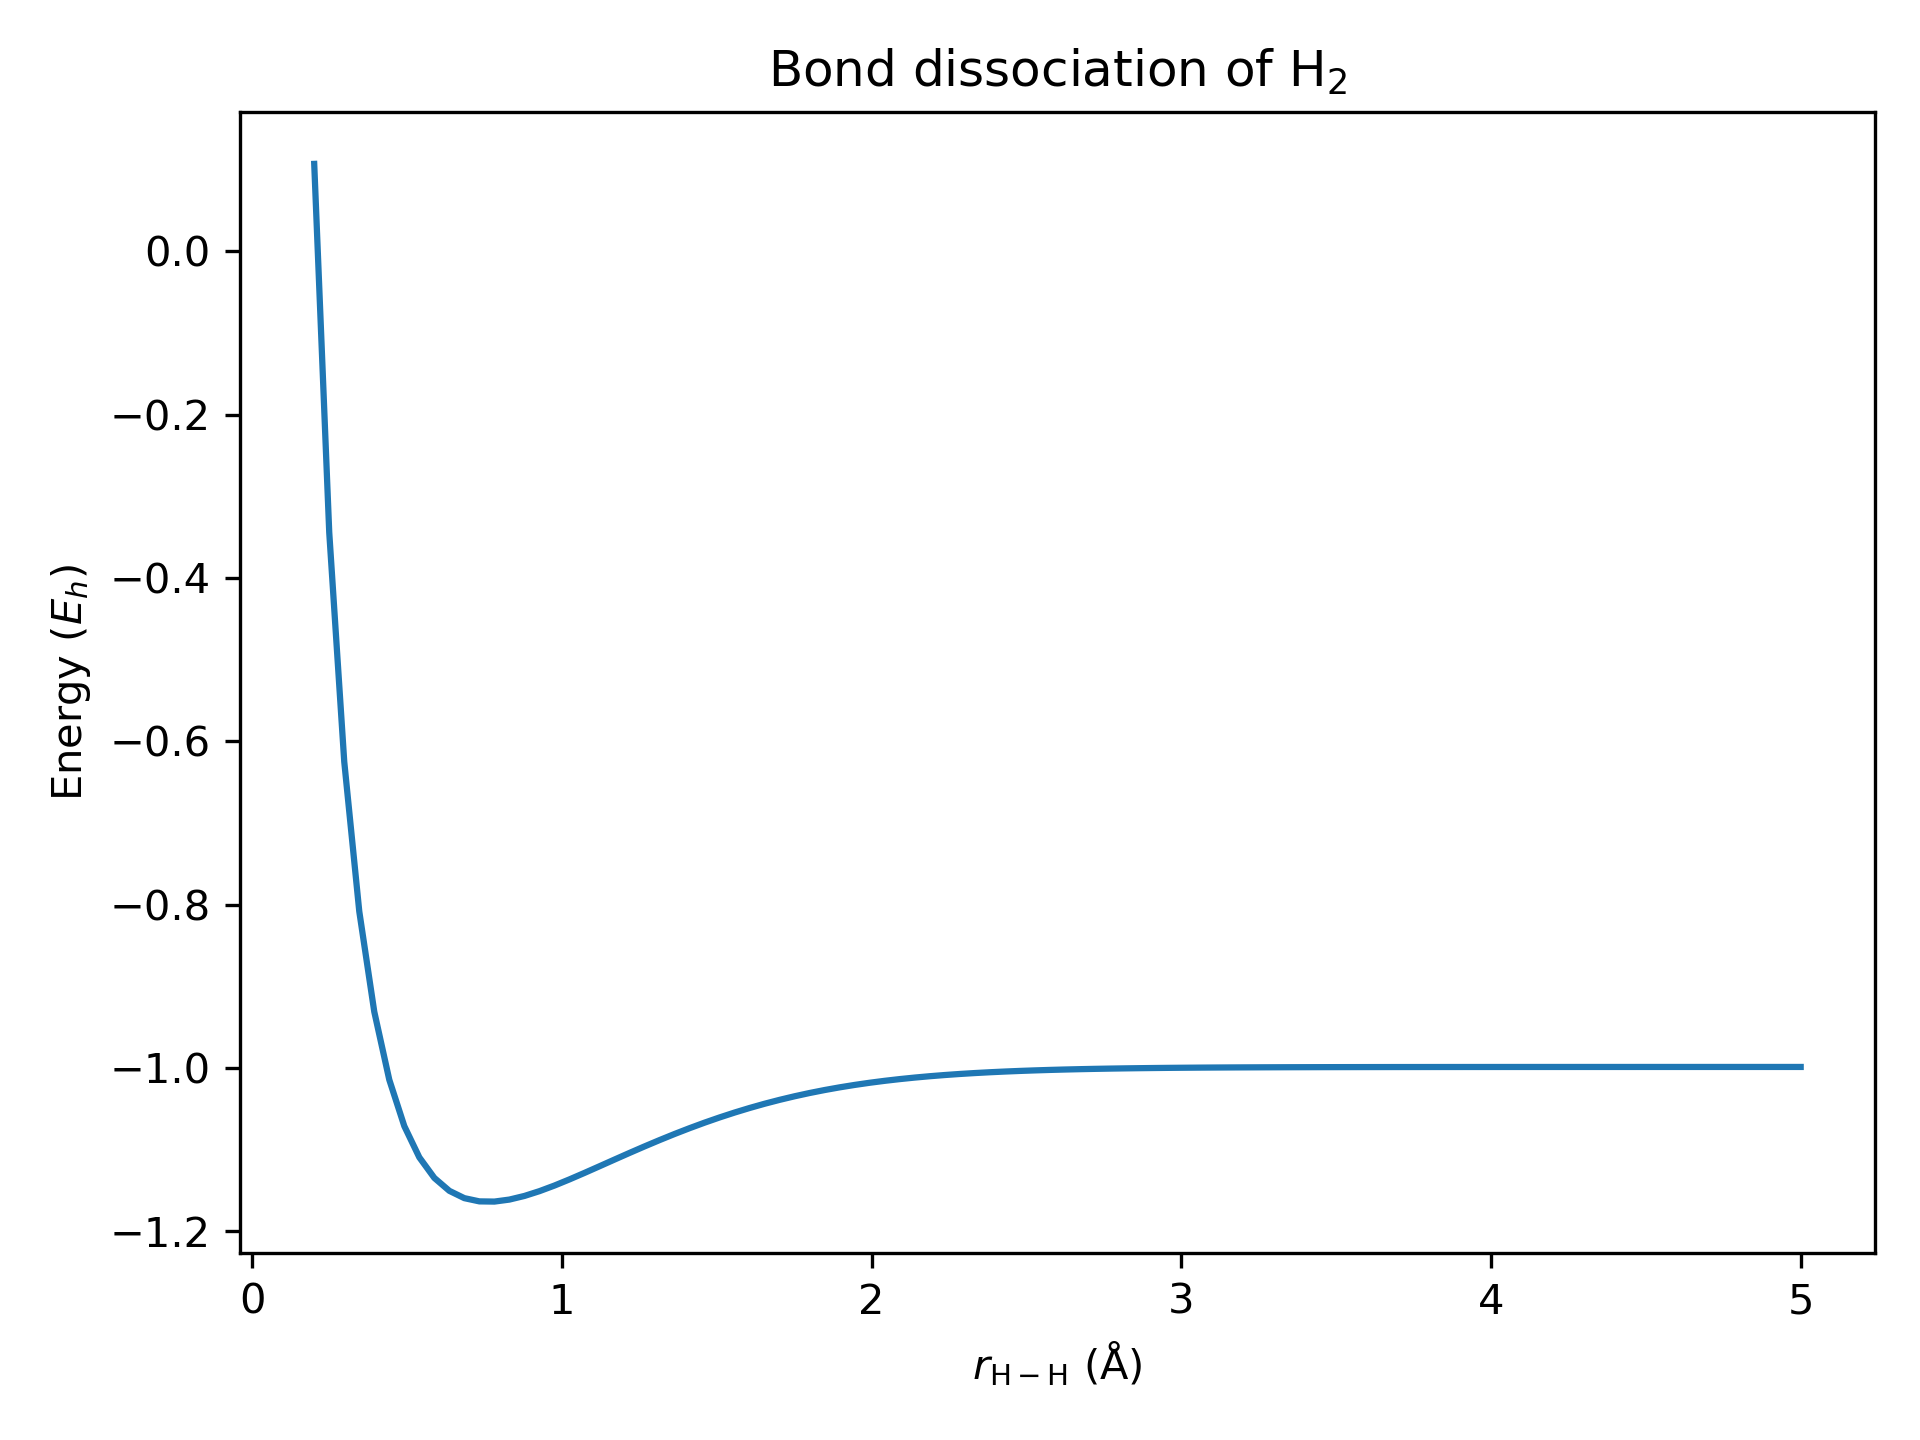
\includegraphics[width=8cm]{h2_dissociation.png}
  \end{center}
\end{frame}

\begin{frame}[fragile]{An example use in scientific: \ce{H2} dissociation}
  To do this, we will:
  \begin{enumerate}
    \item generate a set of input files from \SIrange{0.2}{5}{\angstrom}
    \item compute the corresponding CCSD/cc-pVDZ energies
    \item render the PES plot
  \end{enumerate}
  \pause
  \begin{center}
  \begin{tikzpicture}[
    level 1/.style={sibling distance=10em},
    level 2/.style={sibling distance=4em},
    level 3/.style={sibling distance=2em},
    every node/.style={labelnode, fill=solarized-green!20}]
    \node[fill=solarized-red!20]{h2\_dissociation.png}
    child{node {0.5000.inp.dat}
      child{node{0.5000.inp}}}
    child{node {....inp.dat}
      child{node{...inp}}}
    child{node{5.0000.inp.dat}
      child{node{5.0000.inp}}};

  \end{tikzpicture}
\end{center}
\end{frame}

\begin{frame}{Conclusion}
  Hopefully, I have convinced you that:
  \begin{enumerate}[<+->]
    \item \textco{Make} is not so bad! It is just a bunch of dependency rules
    \item It can help you drive computations efficiently, without rerunning
      stuff twice.
    \item It is a tool that simplifies many different tasks, not only building software
  \end{enumerate}
\end{frame}

\begin{frame}{Related software}
  \begin{enumerate}
  \item \textco{snakemake} {\footnotesize \url{https://snakemake.readthedocs.io/en/stable/index.html}}
  \item \textco{ninja} {\footnotesize \url{https://ninja-build.org/}}
  \item \textco{invoke} {\footnotesize \url{http://www.pyinvoke.org/}}
  \end{enumerate}
\end{frame}

\end{document}